\chapter{Representation Learning}
\label{chapter:representation_learning}
In machine learning, algorithms and learning methods are applied to datasets. Producing useful representations is a crucial step in almost any application that seeks to utilize such datasets quantitatively. Depending on the representation, patterns and explaining regularities in the dataset might be more or less obscured to the model \cite{bengio2013representation}. For this reason, finding a representation that makes such regularities more prominent is often a nontrivial learning task itself. Usually, this involves various preprocessing and cleaning steps of the raw data samples, as well as engineering features that capture the crucial information well. In protein engineering, such cleaning steps may include multiple sequence alignments of protein families and removal of certain noisy/insignificant parts of the protein sequence, while feature engineering could be the step from low-level representation of protein sequences to more abstract features containing fundamental protein properties such as stability and secondary structure. Manually engineering features does not scale well and throttles the application of machine learning models. For this reason, automatically learning suitable representations is a task of major importance in machine learning, often applied internally in a model to transform the input data before passing it to a predicting component such as a classifier. In other cases a machine learning model is built with the sole task of figuring out good representations that can then subsequently be applied to downstream learning tasks as input. Of course, \textit{good} representations depend on the task at hand, but often they will capture abstract, general features of the data. Such representations can often be captured without a task in mind, i.e. by learning from \textit{unsupervised} data. Such representations are discussed in section \ref{sec:supervised_vs_unsupervised}. 

Section \ref{sec:representations} focuses on the task of representing data in machine learning. In probabilistic settings, representations are distributed in a feature space, or \textit{latent space}, such that a given data sample has an associated uncertainty. These representations are discussed in section \ref{seq:latent_space}.

\section{Supervised vs. Unsupervised Learning}
\label{sec:supervised_vs_unsupervised}

A \textit{supervised} learning setting consists of a data set $\prts{x_1, y_1}, \prts{x_2, y_2}, \ldots, \prts{x_n, y_n}$ of $n$ pairs of a data sample $x_i$ and its target $y_i$ (also called a label of the data sample). The learning task is to infer the general function that maps from samples to targets, based on the available data set. This includes unseen samples, and so a successfully learned function generalizes to all samples, not just the observed. In these settings, learned representations has a clear objective; they should aid the supervised learning task. Supervised learning usually requires some processing of data to obtain its associated targets (a supervision), requiring human interaction. This dependency has the undesirable effect that labelled data sets are in many cases expensive and small. Therefore, in many practical settings, supervised learning is a constraint on the size of the available data set, effectively excluding any available data which does not have associated targets. Such constraints can lead to extreme data inefficiency, as in the case of protein sequences shown in figure \ref{fig:data_increase}. Here the Protein Data Bank (PDB) contains the labeled data, in this case the protein sequence and its 3D structure, and UniParc contain raw sequences only. The amount of available unlabeled data is staggering compared to the amount of labeled available data. This difference alone is a strong incentive to explore what we can do in unsupervised learning settings. Even more importantly, the growth of unlabeled protein sequences has so far behaved exponentially, and so we might expect the difference to be even larger in the future.

\begin{figure}[ht]
    \centering
    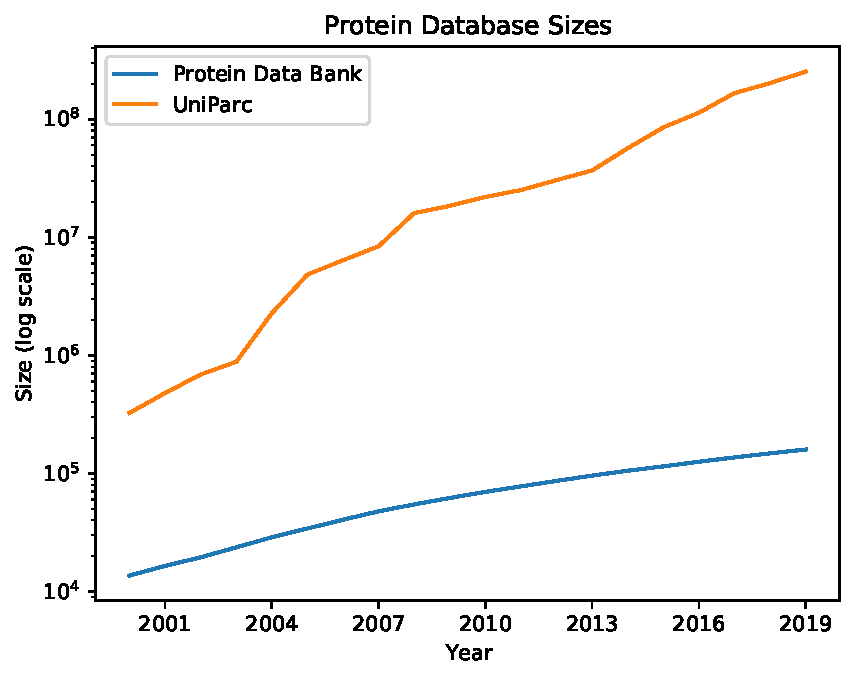
\includegraphics[scale = 0.8]{report/figures/protein_size.pdf}
    \caption{The development of protein database sizes over the last decade. While there is an increase in the size of the Protein Data Bank (from 16,403 in 2001 to 158,985 in 2019), this increase is almost unnoticeable compared to the exponential increase of raw protein sequences in the UniParc database.}
    \label{fig:data_increase}
\end{figure}

In an \textit{unsupervised} learning setting, data samples have no associated targets. The data set is simply $x_1, x_2, \ldots, x_n$ and the learning task is to find underlying structure or pattern in the data samples that is shared across that dataset. Basically, we desire any commonalities or general information in the data set to be reflected in the produced representations. This is typically information such as the distribution of the data set or detection of clusters within the data. This is not trivial, as there is no obvious learning objective, i.e. how does the machine know if it has found anything meaningful when there is no labels to guide the process. In the autoencoding approach, adopted in this thesis and discussed in section \ref{sec:autoencoders}, the unsupervised learning task is simulated by a supervised setting by reconstructing an input data sample from a compressed representation. That is, the data sample is its own target. In the context of representation learning, the underlying assumption is that in order for the model to learn to reconstruct its input from a compressed representation, the representation must necessarily retain properties of the sample that identify it the most. Making the representation compressed is essential, as the model could otherwise naively pass the sample unaltered through its internal components, effectively learning the identity function $f(x) = x$. The model learns to reconstruct the input samples, having the side-effect that it produces internal representations of the data samples. 


% \{discuss this excerpt}
% From \href{https://moalquraishi.wordpress.com/2019/04/01/the-future-of-protein-science-will-not-be-supervised/}{blog}
% \textit{"On the one hand this may seem depressing, but on the other hand, I believe it presents a unique opportunity for unsupervised and semi-supervised machine learning. I am aware of no other problem in which the gap between labelled and unlabeled data is this large and continually increasing. If unsupervised learning can be made to work somewhere, it ought to be here. I emphasize this point because I have followed unsupervised learning with some interest over the last few years, and found most applications to be somewhat uncompelling, in the sense that the increase in performance gained from e.g. unsupervised initialization of an RNN always seems to be marginal. In many applications this is further exacerbated by the fact that acquiring labelled data is not all that expensive, rendering the extra effort that goes into semi-supervised learning even less worthwhile. However, the gap between labelled and unlabelled data in most applications is on the scale of 1 to 2 orders of magnitude, at most. What we see in protein sequence vs. e.g. structure is a gap of 5 orders of magnitude. This suggests, again, that if unsupervised learning were to work anywhere, it ought to be on proteins.}

% \textit{Another advantage of proteins is the wealth of prior knowledge that can be exploited to construct sophisticated loss functions for unsupervised learning, instead of simple next letter prediction (approaches like BERT have gone beyond this, but the amount of unsupervised signals in NLP seem to be much more limited than proteins.)"}

\section{Representations}
\label{sec:representations}
A fundamental assumption in machine learning settings is that hierarchical modelling is possible: explaining aspects of the learning problem can be broken into less and less abstract sub-factors that are ultimately founded in the raw sample input. That is, when we use a machine learning model on a learning task, it represents a hierarchical representation of how the explaining factors of the data is related, starting from concrete, low-level features of the input and becoming gradually more abstract as we pass through the model toward its output. Explaining factors are what a good representation contains, implying that such representations can be learned using neural networks that captures the representation hierarchy.

Another desired property we have on the representation space is that it is smooth: if data samples $x_1$, and $x_2$ are close (by some distance metric), then so are their representations $r(x_1)$ and $r(x_2)$. This is central to the idea that similar samples end up having similar representations. In exploratory settings, this implies that we should look in the neighborhood of a sample if we wish to observe close modifications of that sample.

In addition, any data set we are likely to use is a product of many, complex processes that interact in a shared context. Explanatory factors of the data set are therefore often \textit{entangled}, meaning that they are highly dependent and thus hard to separate (look at independently). Because the data is generated from such complex factors, learning good representations ideally involves \textit{disentangling} them to features that still captures the variation of the data, but are not dependent on each other. Such disentangled representations are however a fundamental impossibility without biases, as shown by \textcite{locatello2018challenging}, indicating that we should not expect to separate causes into neat and separate dimensions in a representation space. Still, representations that contain features that correspond to causes of the observed data may very well generalize to several tasks as these causes are what is assumed to explain the factors of the observed data. The idea is thus that the generality of good representations can be exploited in different supervised learning settings on the same data.

This does not however mean that the learned representation features are easily understood by humans. Usually, representations learned by the deep learning model are complex and hard to interpret. Often, the model is like a black box that somehow figures out how to transform the data into appropriate abstract representations, and those representations are then evaluated based on their metrics/performance, rather than interpretation of what the representations are. Ideally, a good representation also provides this aspect of interpretability for humans.

% statistical strength between learning tasks - information from unsupervised tasks is useful for supervised tasks. idea is to transfer what we have learned by exploiting its generalizability in other settings. "the core idea of representation learning is that the same representation may be useful in both settings"

% a way to leverage unlabeled data

\subsection{Latent Spaces}
\label{seq:latent_space}
% "One hypothesis is that an ideal representation is one in which the features within the representation correspond to the underlying causes of the observed data, with separate features or directions in feature space corresponding to different causes, so that the representation disentangles the causes from one another."

% see DEEPLEARNING p. 533

Here we briefly touch on the idea of modelling explanatory factors using random variables, an idea which is explored in detail in Chapter \ref{chapter:probabilistic_modelling} on probabilistic modelling. As discussed above, if a data sample $\ve{x}$ is generated from a mixture of causes, we can conceptually think of $\ve{x}$ being generated from a mixture model, where each component of the model being a cause for the generating process. As we do not know the underlying mixture model, a way round this is to represent all the explanatory factors by a single (vector) variable. We call this variable $\ve{z}$ a \textit{latent variable}, as we only obtain information about it indirectly through the data, and not from direct observation. The causal generative model for the observed data can then be expressed in terms of $\ve{z}$ as
\[ p(\ve{x}, \ve{z}) = \pxz \pz, \]
where we regard the joint distribution as structured in terms of $\ve{z}$ causing $\ve{x}$, which can be viewed as a simple probabilistic graph model:
\begin{figure}[H]
    \centering
    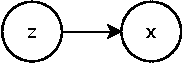
\includegraphics{report/figures/probabilistic_model.pdf}
    % \caption{Caption}
    \label{fig:probabilistic_model_graph}
\end{figure}
The marginal distribution $\px$ can be recovered by integrating over the latent space. The idea is that a good representation is one which recovers the underlying causes represented by $\ve{z}$. Specifically, if we are interested in some property $\ve{y}$ of $\ve{x}$ that is either itself a cause of $\ve{x}$ or related to a cause, the knowledge of $\ve{z}$ can help inferring $p(\ve{y} \mid \ve{x})$, i.e. how likely it is that we have the property $\ve{y}$ given $\ve{x}$.

% semi-supervised learning, transfer learning

\subsection{Protein Representations: Global and Local Representations}
\label{sec:global_local_representations}
The sample space of proteins is very large and governed by a long and arduous evolutionary process. The protein samples observable today in life are distributed in accordance with this process. Making good representations for all proteins is therefore a global representation, i.e. the representation should capture well the core properties and causes of any protein likely to be generated by evolution. A model that can produce such representations would need to be be sufficiently complex to capture the variance of such a vast input space, and the learning task of training such a model is an active research field. The motivation is clear: such representations would be broadly applicable in any setting where proteins are used, regardless of the type of protein. It would also be able to take full advantage of the entire sample space of proteins, as any protein informs such a representation. For much the same reason, the model would be left in the dark for large areas of protein space, as the number of available protein sequences do not evenly cover existing organisms on Earth. It is also questionable whether such a representation would be able to learn truly general properties given that the available protein data is sparse. In addition, most practical protein tasks focus on small sub-regions of protein space, and it is questionable whether a general representation would perform sufficiently well in such settings, compared to a less ambitious, local representation. 

A \textit{local} representation of protein sequences is a representation that is applicable to a subset of proteins, e.g. a protein family, and not the entire global protein space. Such specialized representations have the advantage that they do not need to learn about every single natural protein sequence; this smaller learning task is much more feasible and requires data from the protein subset space alone. The downside is that they do not exploit available data outside of the local space and thus its representations cannot be efficiently used for tasks that rely on data outside the local protein space. In comparison with global representation learning, local representation learning can, all other things being equal, make do with less complex models as the learning task is simpler.

\begin{figure}[ht]
    \centering
    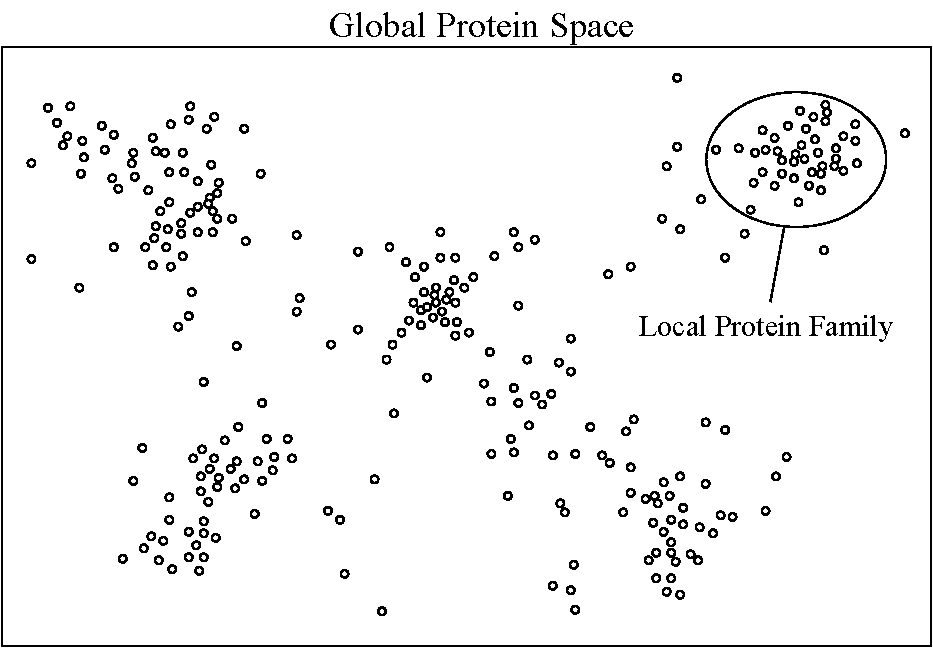
\includegraphics[scale = 0.8]{report/figures/protein_global_local.pdf}
    \caption{A sketch of a space of protein representations in 2 dimensions. The global protein representations (dots) encapsulates all natural protein sequences, while local protein representations are only concerned with a clustered subset, often a protein family.}
    \label{fig:global_local}
\end{figure}

Any natural\footnote{a protein likely to exist in our evolutionary environment, or synthesized proteins derived from occurring proteins} protein share commonalities and causal factors that should help a learner to infer useful information about one protein from another protein. This is irrespective of any global or local distinction, and so a model might preferably in any case first look at all the available protein data (pretrain on global protein space) and then, under task specific conditions finetune on local protein space. In practical settings, the available data under a local space might be sparse, e.g. small protein families with few members. Global pretraining can be the important factor that allow learning to take place from such small datasets.

The usefulness of global versus local representations is an open question, especially in protein representation learning. Global representations seem more generally useful, but also require more training data and more complex models to sufficiently capture the essential features of any given protein. It is also questionable whether global representations for data like proteins are even feasible -- consider this back-of-the-napkin calculation: Let's say that all proteins are approximately 1000 amino acids long, and there are 20 different amino acids. That gives about $1000^{20} = 10^{60}$ potentially possible proteins. Probably only a very small fraction of these are actually possible/useful proteins, so let's just round it down to $10^{20}$ (as a comparison, it is estimated that there are about $10^{80}$ atoms in the universe).

Even with this reduced number of proteins, it seems infeasible for a reasonably sized model to accurately describe so many proteins. That is, a single ``small'' representation should be able to capture all the essential features of all those proteins. If the representation is unable to do this, it may only capture large-scale trends across the global protein space, but fail to capture detail in any local protein space.

In comparison, the local protein space is minuscule. A protein family still contains a lot of proteins, but probably no more than, say, $10^{10}$, and often no more than a few tens of thousand of proteins. Additionally, the proteins in a protein family have more similarities than the proteins of the global space, which means the representation can be simpler, as it only has to concern itself with the remaining differences. Thus, a model utilizing a local representation seems intuitively much more feasible than one using a global representation.

%\{make sure that we explicitly discuss the following: producing global representations, meant to be utilized for the entire space of all proteins, may be too optimistic and performance may suffer in the local protein family landscapes}
% \{discuss this excerpt}
% From \href{https://moalquraishi.wordpress.com/2019/04/01/the-future-of-protein-science-will-not-be-supervised/}{blog}:
%\textit{"A key feature of this type of representation learning is its induction of a global representation of protein sequence space. Much of the prior work in this space has focused on family-specific representations, for example VAE-based ones. While family-specific representations have proven to be very powerful, particularly for protein structure prediction and for predicting the effects of mutant variants, they have always left me feeling somewhat unsatisfied. I say this because from the perspective of data / sampling efficiency, they’re only able to exploit patterns observed within a single protein family. They fragment protein sequence space into local clusters and perform learning, unsupervised or otherwise, separately for each family. This sort of sample vs. model complexity tradeoff is emblematic of much of machine learning, and I’ve written about it before in the context of predicting SH2-mediated protein-protein interactions. On the one hand, if each protein family is learned separately, the complexity of the model is reduced. But the amount of data available is also reduced, fracturing the inherent universality of proteins into tiny phenomenological universes. On the other hand, a global model of protein sequence space is able to leverage all available data, but must learn something truly general, a much more demanding task that substantially increases model complexity. What is the right tradeoff—where is the sweet spot? My hunch has long been that a global model is likely to be more performant. And with UniRep, I believe we’re beginning to see this play out."}

%\textit{"Beyond the question of performance, a global model of protein sequence space has the potential to be much more useful, by being more broadly applicable. The challenge we face in protein informatics, and protein science more broadly, is that our functional characterization of proteins is sparse and patchy. Certain protein families have had the benefit of deep functional characterization, both in terms of gross function (e.g. the plethora of mammalian signaling proteins) and in terms of detailed structural perturbation (e.g. as resultant from deep mutational scans). The GFP family of proteins studied in the UniRep paper is an example of one such family. This patchiness makes it difficult to say something truly useful about the vast majority of proteins (across Prokarya and Eukarya) because, to use an overextended metaphor, they exist in a dark region of sequence space. And the detailed characterization we have of a few families ends up being largely uninformative about this larger space, except in a vague conceptual way."}

%\textit{"Global models of protein sequence space have the potential to change this because, if we can get them to work well, they can at a minimum help us see the connective tissue that underpins protein space, and thereby relate information about well-characterized protein families to poorly characterized ones. In essence, they provide a fancy version of k-nearest neighbors, by densely populating the empty space surrounding sparsely characterized proteins, enabling functional associations to be transferred from one protein to another much farther than previously possible."}

%\textit{"Beyond this, global models of protein sequence hold the possibility of learning something truly general about proteins, that would move us beyond mere k-nearest neighbor matching to something more akin to a linguistics of proteins, decomposing protein sequences into their constituent functional and structural fragments. The fact that UniRep learned something about protein secondary structure is an indication that this is possible and already happening, without any supervision. This is important because unlike secondary structure, most of the principles of protein function (and perhaps structure) remain opaque to us, and so our ability to perform supervision will remain limited for the foreseeable future."}